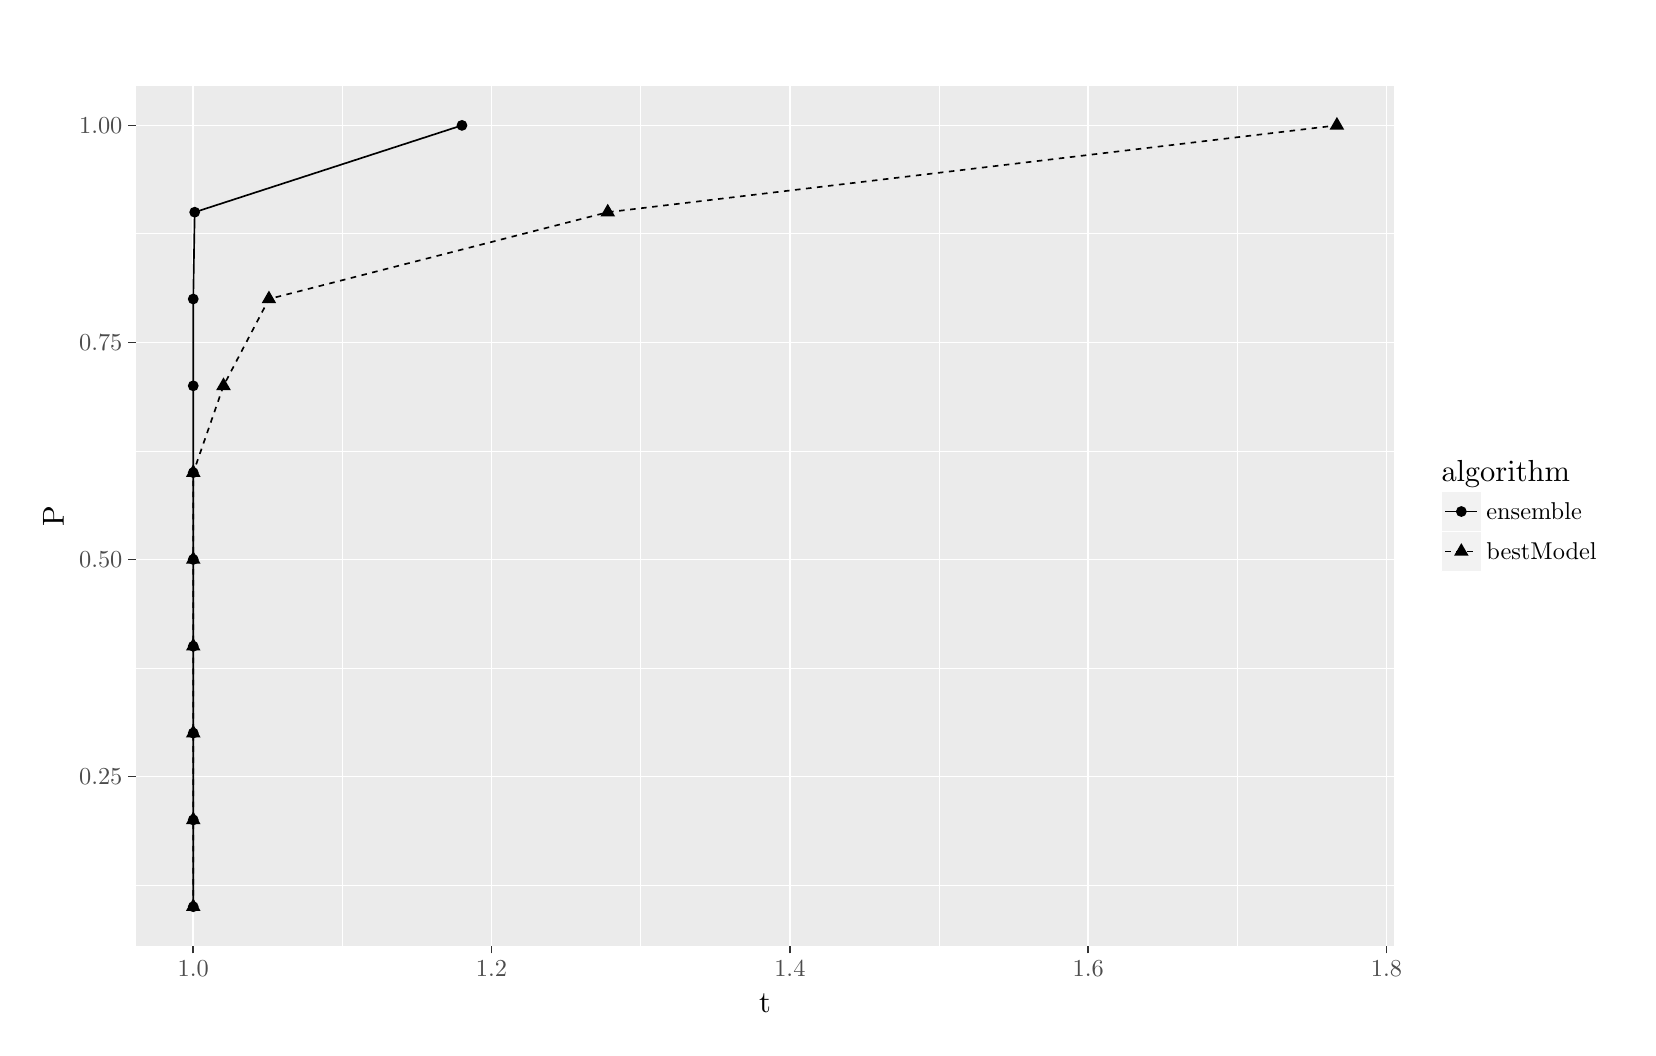
\begin{tikzpicture}[x=1pt,y=1pt]
\definecolor{fillColor}{RGB}{255,255,255}
\path[use as bounding box,fill=fillColor,fill opacity=0.00] (0,0) rectangle (578.16,361.35);
\begin{scope}
\path[clip] (  0.00,  0.00) rectangle (578.16,361.35);
\definecolor{drawColor}{RGB}{255,255,255}
\definecolor{fillColor}{RGB}{255,255,255}

\path[draw=drawColor,line width= 0.6pt,line join=round,line cap=round,fill=fillColor] (  0.00, -0.00) rectangle (578.16,361.35);
\end{scope}
\begin{scope}
\path[clip] ( 39.17, 29.59) rectangle (493.75,340.16);
\definecolor{fillColor}{gray}{0.92}

\path[fill=fillColor] ( 39.17, 29.59) rectangle (493.75,340.16);
\definecolor{drawColor}{RGB}{255,255,255}

\path[draw=drawColor,line width= 0.3pt,line join=round] ( 39.17, 51.55) --
	(493.75, 51.55);

\path[draw=drawColor,line width= 0.3pt,line join=round] ( 39.17,129.97) --
	(493.75,129.97);

\path[draw=drawColor,line width= 0.3pt,line join=round] ( 39.17,208.40) --
	(493.75,208.40);

\path[draw=drawColor,line width= 0.3pt,line join=round] ( 39.17,286.83) --
	(493.75,286.83);

\path[draw=drawColor,line width= 0.3pt,line join=round] (113.73, 29.59) --
	(113.73,340.16);

\path[draw=drawColor,line width= 0.3pt,line join=round] (221.52, 29.59) --
	(221.52,340.16);

\path[draw=drawColor,line width= 0.3pt,line join=round] (329.31, 29.59) --
	(329.31,340.16);

\path[draw=drawColor,line width= 0.3pt,line join=round] (437.11, 29.59) --
	(437.11,340.16);

\path[draw=drawColor,line width= 0.6pt,line join=round] ( 39.17, 90.76) --
	(493.75, 90.76);

\path[draw=drawColor,line width= 0.6pt,line join=round] ( 39.17,169.19) --
	(493.75,169.19);

\path[draw=drawColor,line width= 0.6pt,line join=round] ( 39.17,247.61) --
	(493.75,247.61);

\path[draw=drawColor,line width= 0.6pt,line join=round] ( 39.17,326.04) --
	(493.75,326.04);

\path[draw=drawColor,line width= 0.6pt,line join=round] ( 59.83, 29.59) --
	( 59.83,340.16);

\path[draw=drawColor,line width= 0.6pt,line join=round] (167.62, 29.59) --
	(167.62,340.16);

\path[draw=drawColor,line width= 0.6pt,line join=round] (275.42, 29.59) --
	(275.42,340.16);

\path[draw=drawColor,line width= 0.6pt,line join=round] (383.21, 29.59) --
	(383.21,340.16);

\path[draw=drawColor,line width= 0.6pt,line join=round] (491.00, 29.59) --
	(491.00,340.16);
\definecolor{drawColor}{RGB}{0,0,0}

\path[draw=drawColor,line width= 0.6pt,line join=round] ( 59.83, 43.70) --
	( 59.83, 75.07) --
	( 59.83,106.45) --
	( 59.83,137.82) --
	( 59.83,169.19) --
	( 59.83,200.56) --
	( 59.83,231.93) --
	( 59.83,263.30) --
	( 60.35,294.67) --
	(156.93,326.04);

\path[draw=drawColor,line width= 0.6pt,dash pattern=on 2pt off 2pt ,line join=round] ( 59.83, 43.70) --
	( 59.83, 75.07) --
	( 59.83,106.45) --
	( 59.83,137.82) --
	( 59.83,169.19) --
	( 59.84,200.56) --
	( 70.76,231.93) --
	( 87.18,263.30) --
	(209.61,294.67) --
	(473.09,326.04);
\definecolor{fillColor}{RGB}{0,0,0}

\path[fill=fillColor] ( 59.83, 43.70) circle (  1.96);

\path[fill=fillColor] ( 59.83, 75.07) circle (  1.96);

\path[fill=fillColor] ( 59.83,106.45) circle (  1.96);

\path[fill=fillColor] ( 59.83,137.82) circle (  1.96);

\path[fill=fillColor] ( 59.83,169.19) circle (  1.96);

\path[fill=fillColor] ( 59.83,200.56) circle (  1.96);

\path[fill=fillColor] ( 59.83,231.93) circle (  1.96);

\path[fill=fillColor] ( 59.83,263.30) circle (  1.96);

\path[fill=fillColor] ( 60.35,294.67) circle (  1.96);

\path[fill=fillColor] (156.93,326.04) circle (  1.96);

\path[fill=fillColor] ( 59.83, 46.75) --
	( 62.47, 42.18) --
	( 57.19, 42.18) --
	cycle;

\path[fill=fillColor] ( 59.83, 78.13) --
	( 62.47, 73.55) --
	( 57.19, 73.55) --
	cycle;

\path[fill=fillColor] ( 59.83,109.50) --
	( 62.47,104.92) --
	( 57.19,104.92) --
	cycle;

\path[fill=fillColor] ( 59.83,140.87) --
	( 62.47,136.29) --
	( 57.19,136.29) --
	cycle;

\path[fill=fillColor] ( 59.83,172.24) --
	( 62.47,167.66) --
	( 57.19,167.66) --
	cycle;

\path[fill=fillColor] ( 59.84,203.61) --
	( 62.48,199.03) --
	( 57.19,199.03) --
	cycle;

\path[fill=fillColor] ( 70.76,234.98) --
	( 73.40,230.40) --
	( 68.12,230.40) --
	cycle;

\path[fill=fillColor] ( 87.18,266.35) --
	( 89.82,261.77) --
	( 84.54,261.77) --
	cycle;

\path[fill=fillColor] (209.61,297.72) --
	(212.26,293.15) --
	(206.97,293.15) --
	cycle;

\path[fill=fillColor] (473.09,329.09) --
	(475.73,324.52) --
	(470.45,324.52) --
	cycle;
\end{scope}
\begin{scope}
\path[clip] (  0.00,  0.00) rectangle (578.16,361.35);
\definecolor{drawColor}{gray}{0.30}

\node[text=drawColor,anchor=base east,inner sep=0pt, outer sep=0pt, scale=  0.88] at ( 34.22, 87.73) {0.25};

\node[text=drawColor,anchor=base east,inner sep=0pt, outer sep=0pt, scale=  0.88] at ( 34.22,166.16) {0.50};

\node[text=drawColor,anchor=base east,inner sep=0pt, outer sep=0pt, scale=  0.88] at ( 34.22,244.58) {0.75};

\node[text=drawColor,anchor=base east,inner sep=0pt, outer sep=0pt, scale=  0.88] at ( 34.22,323.01) {1.00};
\end{scope}
\begin{scope}
\path[clip] (  0.00,  0.00) rectangle (578.16,361.35);
\definecolor{drawColor}{gray}{0.20}

\path[draw=drawColor,line width= 0.6pt,line join=round] ( 36.42, 90.76) --
	( 39.17, 90.76);

\path[draw=drawColor,line width= 0.6pt,line join=round] ( 36.42,169.19) --
	( 39.17,169.19);

\path[draw=drawColor,line width= 0.6pt,line join=round] ( 36.42,247.61) --
	( 39.17,247.61);

\path[draw=drawColor,line width= 0.6pt,line join=round] ( 36.42,326.04) --
	( 39.17,326.04);
\end{scope}
\begin{scope}
\path[clip] (  0.00,  0.00) rectangle (578.16,361.35);
\definecolor{drawColor}{gray}{0.20}

\path[draw=drawColor,line width= 0.6pt,line join=round] ( 59.83, 26.84) --
	( 59.83, 29.59);

\path[draw=drawColor,line width= 0.6pt,line join=round] (167.62, 26.84) --
	(167.62, 29.59);

\path[draw=drawColor,line width= 0.6pt,line join=round] (275.42, 26.84) --
	(275.42, 29.59);

\path[draw=drawColor,line width= 0.6pt,line join=round] (383.21, 26.84) --
	(383.21, 29.59);

\path[draw=drawColor,line width= 0.6pt,line join=round] (491.00, 26.84) --
	(491.00, 29.59);
\end{scope}
\begin{scope}
\path[clip] (  0.00,  0.00) rectangle (578.16,361.35);
\definecolor{drawColor}{gray}{0.30}

\node[text=drawColor,anchor=base,inner sep=0pt, outer sep=0pt, scale=  0.88] at ( 59.83, 18.58) {1.0};

\node[text=drawColor,anchor=base,inner sep=0pt, outer sep=0pt, scale=  0.88] at (167.62, 18.58) {1.2};

\node[text=drawColor,anchor=base,inner sep=0pt, outer sep=0pt, scale=  0.88] at (275.42, 18.58) {1.4};

\node[text=drawColor,anchor=base,inner sep=0pt, outer sep=0pt, scale=  0.88] at (383.21, 18.58) {1.6};

\node[text=drawColor,anchor=base,inner sep=0pt, outer sep=0pt, scale=  0.88] at (491.00, 18.58) {1.8};
\end{scope}
\begin{scope}
\path[clip] (  0.00,  0.00) rectangle (578.16,361.35);
\definecolor{drawColor}{RGB}{0,0,0}

\node[text=drawColor,anchor=base,inner sep=0pt, outer sep=0pt, scale=  1.10] at (266.46,  5.50) {t};
\end{scope}
\begin{scope}
\path[clip] (  0.00,  0.00) rectangle (578.16,361.35);
\definecolor{drawColor}{RGB}{0,0,0}

\node[text=drawColor,rotate= 90.00,anchor=base,inner sep=0pt, outer sep=0pt, scale=  1.10] at ( 13.08,184.87) {P};
\end{scope}
\begin{scope}
\path[clip] (  0.00,  0.00) rectangle (578.16,361.35);
\definecolor{fillColor}{RGB}{255,255,255}

\path[fill=fillColor] (505.13,159.13) rectangle (572.66,210.61);
\end{scope}
\begin{scope}
\path[clip] (  0.00,  0.00) rectangle (578.16,361.35);
\definecolor{drawColor}{RGB}{0,0,0}

\node[text=drawColor,anchor=base west,inner sep=0pt, outer sep=0pt, scale=  1.10] at (510.82,197.35) {algorithm};
\end{scope}
\begin{scope}
\path[clip] (  0.00,  0.00) rectangle (578.16,361.35);
\definecolor{drawColor}{RGB}{255,255,255}
\definecolor{fillColor}{gray}{0.95}

\path[draw=drawColor,line width= 0.6pt,line join=round,line cap=round,fill=fillColor] (510.82,179.28) rectangle (525.28,193.73);
\end{scope}
\begin{scope}
\path[clip] (  0.00,  0.00) rectangle (578.16,361.35);
\definecolor{drawColor}{RGB}{0,0,0}

\path[draw=drawColor,line width= 0.6pt,line join=round] (512.27,186.51) -- (523.83,186.51);
\end{scope}
\begin{scope}
\path[clip] (  0.00,  0.00) rectangle (578.16,361.35);
\definecolor{fillColor}{RGB}{0,0,0}

\path[fill=fillColor] (518.05,186.51) circle (  1.96);
\end{scope}
\begin{scope}
\path[clip] (  0.00,  0.00) rectangle (578.16,361.35);
\definecolor{drawColor}{RGB}{255,255,255}
\definecolor{fillColor}{gray}{0.95}

\path[draw=drawColor,line width= 0.6pt,line join=round,line cap=round,fill=fillColor] (510.82,164.82) rectangle (525.28,179.28);
\end{scope}
\begin{scope}
\path[clip] (  0.00,  0.00) rectangle (578.16,361.35);
\definecolor{drawColor}{RGB}{0,0,0}

\path[draw=drawColor,line width= 0.6pt,dash pattern=on 2pt off 2pt ,line join=round] (512.27,172.05) -- (523.83,172.05);
\end{scope}
\begin{scope}
\path[clip] (  0.00,  0.00) rectangle (578.16,361.35);
\definecolor{fillColor}{RGB}{0,0,0}

\path[fill=fillColor] (518.05,175.10) --
	(520.69,170.53) --
	(515.41,170.53) --
	cycle;
\end{scope}
\begin{scope}
\path[clip] (  0.00,  0.00) rectangle (578.16,361.35);
\definecolor{drawColor}{RGB}{0,0,0}

\node[text=drawColor,anchor=base west,inner sep=0pt, outer sep=0pt, scale=  0.88] at (527.09,183.47) {ensemble};
\end{scope}
\begin{scope}
\path[clip] (  0.00,  0.00) rectangle (578.16,361.35);
\definecolor{drawColor}{RGB}{0,0,0}

\node[text=drawColor,anchor=base west,inner sep=0pt, outer sep=0pt, scale=  0.88] at (527.09,169.02) {bestModel};
\end{scope}
\end{tikzpicture}

